\documentclass[conference]{IEEEtran}

\usepackage{cite}
\usepackage{amsmath,amssymb,amsfonts}
\usepackage{algorithmic}
\usepackage{graphicx}
\usepackage{textcomp}
\usepackage{xcolor}
\usepackage{fontawesome}
\usepackage{siunitx}
\usepackage[hidelinks]{hyperref}
\usepackage{url}

\begin{document}

    \title{Virtual Reality Assignment}

    \author{\IEEEauthorblockN{wcrr51}
    \IEEEauthorblockA{\textit{Department of Computer Science} \\
    \textit{Durham University}\\
    Durham, United Kingdom \\
    wcrr51@durham.ac.uk}}

    \maketitle
    
    \begin{abstract}
        This report looks at designing, implementing and evaluating a Virtual Reality (VR) lens distortion correction system.
    \end{abstract}
    
    \begin{IEEEkeywords}
        Virtual reality, lens distortion, distortion correction.
    \end{IEEEkeywords}

    \section{Introduction}\label{sec:introduction}
    Head-mounted displays (HMDs) represent the current state of the art in virtual reality (VR).
As the user requires a wide field of view (FOV) for immersion, lenses are used to project the emitted image (from the near-by screen) into the eye, making the image appear larger and further away.

However, the real-world physical properties of these lenses incur the introduction of visible distortions and optical aberrations.
The class of these that will be considered in this paper are referred to as radial distortions.
These distortions are rotation-wise invariant (about the centre of the image) and vary only in their radius.

One such example of these is pincushion distortion.
Pincushion distortion appears as the stretching of objects the further they are from the centre of the lens, causing the corners of the image to become more \textit{pointed} (hence a cushion shape as shown in Fig.~\ref{fig:distortion} (a)).
Playing in VR with this can quickly become disorientating or nauseating due to greater acceleration of object towards the periphery compared to the centre.

In order to correct for pincushion distortion, the opposite distortion can be used.
This conversely causes objects to become more compressed (or magnified) the further away they are from the origin, making the corners more \textit{rounded}.
Because of this appearance, it is called barrel distortion (Fig.~\ref{fig:distortion} (b)).

Another example that will be briefly considered is lateral chromatic aberration (LCA).
Unlike longitudinal chromatic aberration, that causes a colour-variant blurriness across the whole image, LCA causes a fringing between colours dependent on how far they are from the centre of the lens.
This is most visible towards the corners of an image appearing as colour-fringing on edges or high contrast areas.
LCA is caused by the fact that since the different colours have different wavelengths, they are refracted differently to each other, meaning, for a given lens, they have a different focal point.
This is shown in Fig.~\ref{fig:chromatic-aberration}.

\begin{figure}[ht]
    \centering
    \subfloat[Pincushion Distortion]{
\includegraphics[width=0.225\textwidth]{figures/pincushion}}
    \hfil
    \subfloat[Barrel Distortion]{
\includegraphics[width=0.225\textwidth]{figures/barrel}}
    \caption{Barrel and pincushion distortion (by WolfWings for Wikipedia, USPD 2008).}
    \label{fig:distortion}
\end{figure}

\begin{figure}[ht]
    \centering
    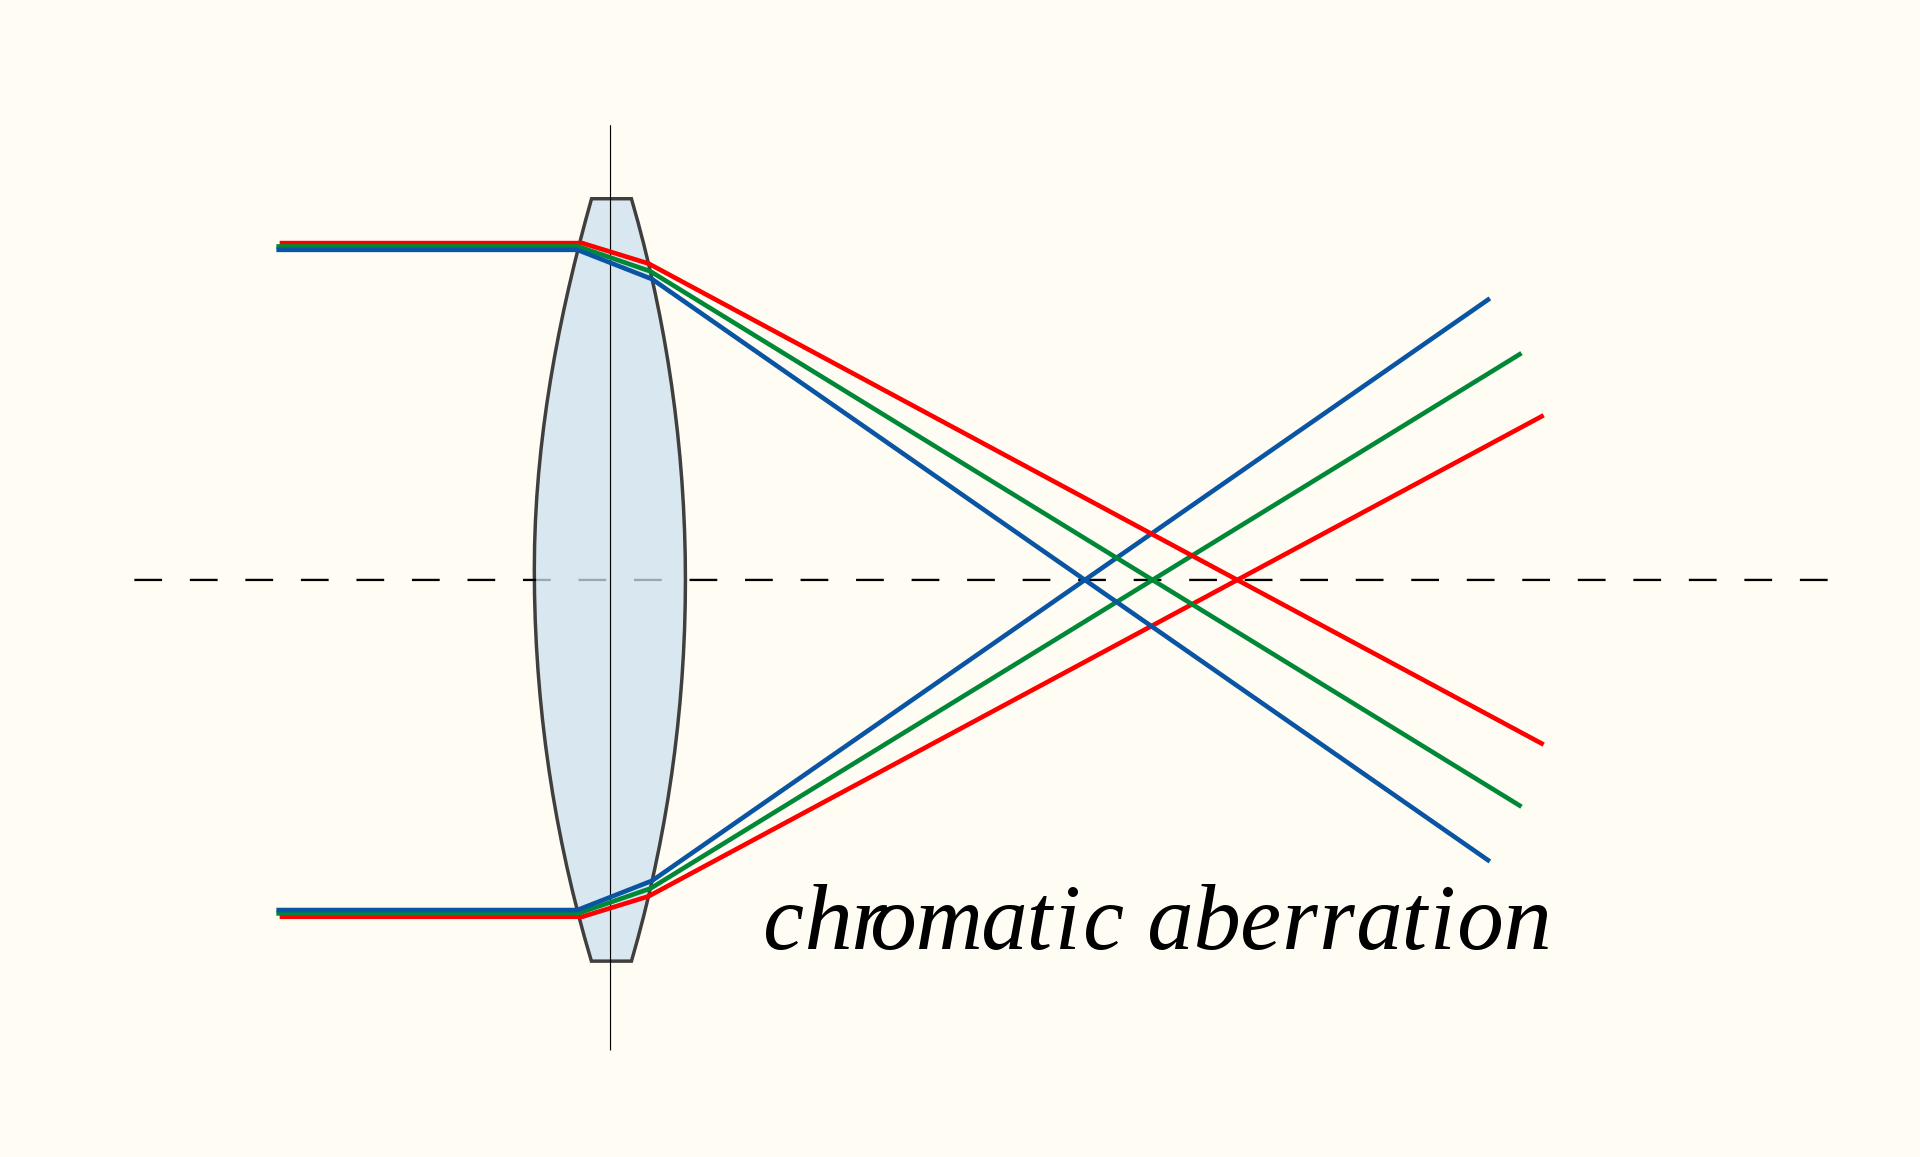
\includegraphics[width=0.4\textwidth]{figures/ca}
    \caption{Diagram of chromatic aberration (by Bob Mellish for Wikipedia, CC 2006).}
    \label{fig:chromatic-aberration}
\end{figure}


    ~\cite{brown1966decentering}

    \bibliographystyle{IEEEtran}
    \bibliography{references}
    \vspace{12pt}
    \color{red}

\end{document}
